\documentclass[aspectratio=169]{beamer}
\usepackage{amsmath}
\usepackage{amssymb}
\usepackage{amsfonts}
\usepackage{graphicx}
\usepackage{luatexja} 
\usepackage{comment}
\usepackage{bm}
\usepackage{setspace}
\usepackage{caption}
\usepackage{xcolor}
\usepackage[numbers]{natbib}
\usepackage{tikz}
\usetheme{metropolis}
\usefonttheme{default}
%\usetheme{LightTheme}
\setbeamertemplate{footline}[framenumber]
\setbeamertemplate{caption}[numbered]
\setbeamertemplate{navigation symbols}{}
\setlength{\baselineskip}{10pt}
\setbeamertemplate{bibliography item}{}
% プリアンブルに追加
\setbeamercolor{block title}{bg=green!50, fg=black} % タイトル背景は薄緑、文字は黒
\setbeamercolor{block body}{bg=green!10, fg=black}  % 本文背景も薄緑、文字は黒
\setbeamertemplate{blocks}[rounded][shadow=false]     % 角丸にして影なし
\begin{document}

% タイトルフレーム
\title{木幅学習システムの構築}
\subtitle{高効率なグラフ解析に向けた木幅概念の学習システム構築}
\author{明治大学理工学部情報科学科\\ 小林紹子\quad 玉木久夫\quad 井口幸洋} % 必要に応じて変更・削除
\date{\today} % 必要に応じて変更・削除

\begin{frame}[plain]
  \titlepage

  \begin{tikzpicture}[remember picture,overlay]
    \node[
      anchor=south east,
      xshift=-0.6cm,
      yshift=0cm
    ] at (current page.south east)
    {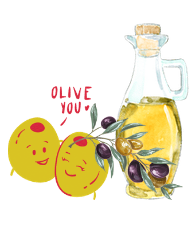
\includegraphics[width=3.8cm]{olive.png}};
  \end{tikzpicture}

\end{frame}

\begin{frame}{目次}
  % セクションは標準の番号付け
  \setbeamertemplate{section in toc}[sections numbered]
  
  % サブセクションを「親番号.子番号」にカスタマイズ
  \setbeamertemplate{subsection in toc}{%
    \leavevmode\leftskip=3em% 左側のインデント（下げ幅）
    \inserttocsectionnumber.\inserttocsubsectionnumber% 「3.1」の部分
    \hspace{1em}% 番号とタイトルの間のスペース
    \inserttocsubsection\par
  }
  
  \tableofcontents
\end{frame}

\section{はじめに}
\begin{frame}{はじめに}
	\begin{itemize}
		\setlength{\parskip}{1em}
		\item グラフ理論\cite{wilson1979introduction}は,ディペンダブルコンピューティング分野における信頼性解析など,多くの分野で基礎理論として用いられる.
		\item 一般に,解くことが困難な問題であっても,対象となるグラフが木構造であれば,容易に解けることが知られている.
		\item 木分解,木幅はグラフ理論やアルゴリズム設計で重要な概念である.
		\item 木分解・木幅の認知度が低い原因
		
		      \begin{itemize}
			      \setlength{\parskip}{0.5em}
			      \item 理解が難しい（定義が具体的にイメージしにくい, 木分解の構築の難しさ）.
			      \item 日本語で学べる教材や可視化・インタラクティブな教材が少ない.
		      \end{itemize}
		\item \textbf{\Rightarrow 木幅や木分解の定義理解を促進する学習システムを開発}
	\end{itemize}


\end{frame}





\section{木と閉路}
\begin{frame}{木と閉路}
	\begin{columns}
		\begin{column}{0.58\textwidth}
			\begin{itemize}
				\setlength{\parskip}{0.5em}
				\item 閉路：\\始点と終点が一致し,それ以外の頂点を重複せずに通る道.
				\item 木：\\閉路を含まず,連結である無向グラフ\cite{wilson1979introduction}.
				\item 木の特徴
				      \begin{itemize}
					      \setlength{\parskip}{0.5em}
					      \item 任意の2頂点間にただ一つの単純路が存在\cite{bondy1976graph}.
					      \item 任意の辺を一つ削除すると,木は複数の連結成分に分裂.
				      \end{itemize}
			\end{itemize}
		\end{column}
		\begin{column}{0.48\textwidth}
			\begin{figure}
				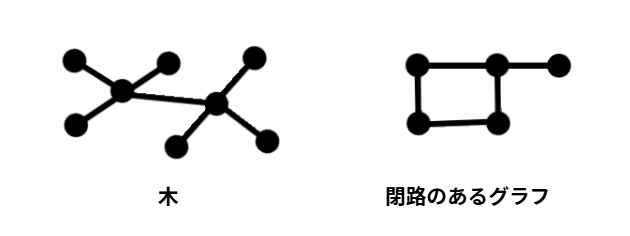
\includegraphics[scale = 0.4]{tree.png}
				\caption{木と閉路}
				\vspace{1.5em}
				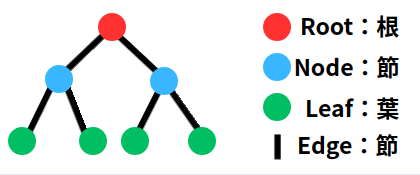
\includegraphics[scale = 0.45]{tree_instruction.png}
				\caption{木構造の用語}
			\end{figure}
		\end{column}
	\end{columns}

\end{frame}

\begin{frame}{木構造はなぜ扱いやすいか}
\begin{itemize}
  \setlength{\parskip}{1em}

  \item 木は閉路を持たず，構造が単純.
  \item 頂点や辺を削除すると，自然にグラフが分割される.
  \item \Rightarrow 再帰構造を持ち，動的計画法が適用しやすい.

  \item 一方，一般のグラフは閉路を含み，
        木と同様のアルゴリズムの適用は困難.

\vspace{1.5em}
\end{itemize}
		\centering
	  \textbf{一般グラフを「木に近い構造」として扱う枠組み \quad \Rrightarrow \quad \color{blue}{木分解}}\\
    {\tiny N. Robertson and P. D. Seymour, ``Graph minors. II. Algorithmic aspects of tree-width,'' \textit{Journal of Algorithms}, vol. 7, no. 3, pp. 309--322, 1986.}
  
\vspace{1em}
\footnotesize{
\begin{itemize}
    \item \textbf{起源}: 1976年に \alert{Halin} が \alert{$S$-functions} を定義．無限グラフの端（ends）を分離する構造として，現在の木分解と実質的に同等の概念を初めて提唱した．
    \item \textbf{確立}: 1986年に \alert{Robertson \& Seymour} が \alert{木分解} として再定義．グラフ・マイナー定理の証明に導入し，同時にNP困難な問題へのアルゴリズム的有用性を確立した．
}
\end{itemize}
\end{frame}

\section{木分解（tree decomposition）}
\begin{frame}{木分解（tree decomposition）とは}
	\textbf{木分解：}
	\\一般のグラフの頂点集合を部分集合の集まりとして分割し,木構造で表現する.
\vspace{1em}
\begin{block}{木分解の定義}
グラフ $G=(V,E)$ に対し，
木 $T=(I,F)$ とバッグ集合 $\{X_i \mid i\in I\}$ が
次を満たすとき，これを\textbf{木分解}という\cite{robertson1986graph}．
\vspace{1em}
\begin{itemize}
  \setlength{\leftskip}{2em}
  \setlength{\parskip}{0.4em}
  \item[(TD1)] すべての頂点はどこかのバッグに含まれる.
  \item[(TD2)] すべての辺の両端は同じバッグに含まれる.
  \item[(TD3)] 同じ頂点を含むバッグは木 $T$ 上で連結である.
\end{itemize}
\vspace{1.5em}
\end{block}
\end{frame}

\begin{frame}{木分解の例}
	\begin{block}{}
	\begin{itemize}
		\setlength{\leftskip}{1em}
    \setlength{\parskip}{0.2em}
	\footnotesize{
  \item[(TD1)] すべての頂点はどこかのバッグに含まれる. 
  \item[(TD2)] すべての辺の両端は同じバッグに含まれる. 
  \item[(TD3)] 同じ頂点を含むバッグは木 $T$ 上で連結である.（点線）
  }
\end{itemize}
	\end{block}
	\begin{columns}
  \begin{column}{0.45\textwidth}
    \begin{figure}
      \centering
      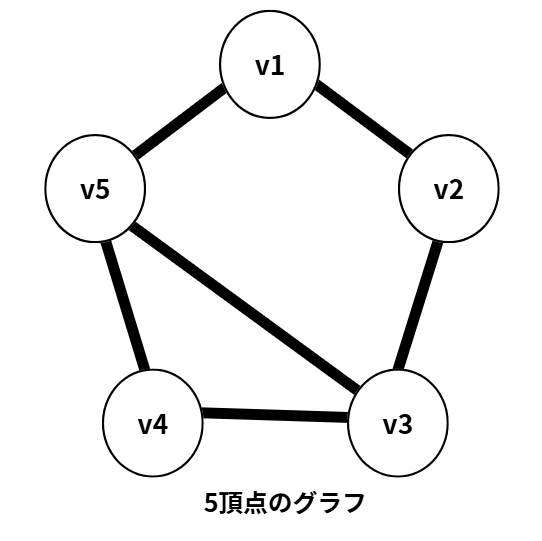
\includegraphics[height=0.6\textheight]{5-nodes-tree-diagrams.png}
      \caption{例}
			\label{5-nodes-graph}
    \end{figure}
  \end{column}

  \begin{column}{0.55\textwidth}
    \begin{figure}
      \centering
      
\includegraphics[height=0.6\textheight]{tree-decomposition-rule.png}
      \caption{左図のグラフの木分解の例}
			\label{5-nodes-tree-decomposition}
    \end{figure}
	\end{column}
	\end{columns}
\end{frame}

\section{木幅（treewidth）}
\begin{frame}{木幅（treewidth）とは}
\begin{itemize}
  \setlength{\parskip}{1em}
  \item 木分解において重要なのは「部分集合の大きさ」＝「バッグの大きさ」.
  \item この大きさを「幅（width）」という.
  \item バッグが小さいほど，木に近い構造を持つと考えられる.
\end{itemize}

\vspace{1em}

\begin{block}{木分解の幅の定義}
\[
\max_{i\in I} (|X_i|-1)
\]
\end{block}

\vspace{2em}
\begin{block}{木幅の定義}
	\centering
すべての場合における木分解の幅の最小値.
\end{block}
\end{frame}

\begin{frame}{木分解と木幅の例}
\begin{columns}
  \begin{column}{0.45\textwidth}
    \begin{figure}
      \centering
      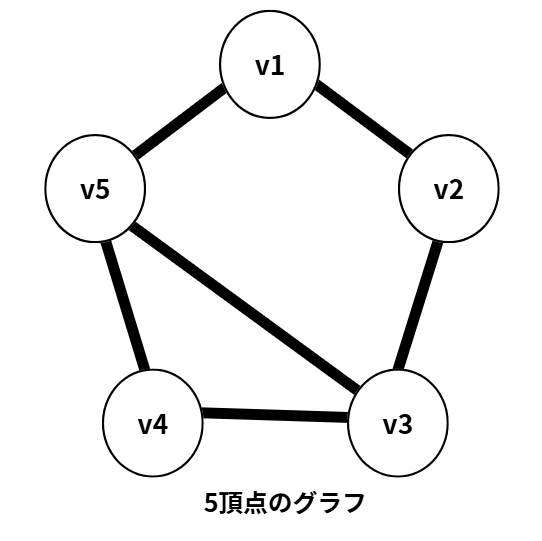
\includegraphics[height=0.6\textheight]{5-nodes-tree-diagrams.png}
      \caption*{例（再掲）}
    \end{figure}
  \end{column}

  \begin{column}{0.55\textwidth}
    \begin{figure}
      \centering
      
\includegraphics[height=0.6\textheight]{tree-decomposition-rule.png}
      \caption*{左図のグラフの木分解の例（再掲）}
    \end{figure}

    \vspace{0.5em}
    
  \end{column}
\end{columns}
\centering{
各バッグの大きさ：3\qquad \qquad 幅：$3-1=2$\\
\Rightarrow 他の木分解も考慮した結果,このグラフの木幅は2となる.
}
\end{frame}

\section{木幅学習システムの開発}

\begin{frame}{設計方針}

% ---- このフレーム内だけ色を変更 ----
\setbeamercolor{block title}{bg=orange!35, fg=black}
\setbeamercolor{block body}{bg=orange!15, fg=black}

\begin{block}{設計方針}
\begin{itemize}
  \setlength{\parskip}{0.6em}
  \item 木分解の定義や性質を「問題形式」で確認.
  \item 理解度を即時に確認できる構成.
  \item 問題の難易度を段階的に上げ，定義理解から応用へ.
  \item グラフや木構造をインタラクティブに選択可能.
\end{itemize}
\vspace{0.3em}
\end{block}

\vspace{0.5em}

\begin{block}{特徴}
\begin{itemize}
  \setlength{\parskip}{0.6em}
  \item 木分解の構築を直接求めず，定義理解に必要な前提知識を段階的に獲得.
  \item 木構造の頂点・辺情報を保持するため，グラフを画像でなくツールで生成.
\end{itemize}
\vspace{0.3em}
\end{block}

\end{frame}

\begin{frame}{使用技術と実装状況}

\setbeamercolor{block title}{bg=orange!35, fg=black}
\setbeamercolor{block body}{bg=orange!15, fg=black}

\begin{columns}[T] % 上揃え
  % ===== 左カラム =====
  \begin{column}{0.6\textwidth}
    \begin{block}{使用技術}
      \begin{itemize}
        \setlength{\parskip}{0.3em}
        \item \textbf{Node.js}：
              サーバ側でJavaScriptを実行\cite{nodejs}.
        \item \textbf{TypeScript}：
              型付けによる安全性向上\cite{TypeScript}.
        \item \textbf{Next.js / React}：
              動的で管理しやすいUI構築\cite{Next.js,React/Next.js,React,React2025}.
        \item \textbf{SQLite + Prisma}：
              軽量DBとORMによるデータ管理\cite{sqlite,Prisma}.
        \item \textbf{ReactFlow}：
              グラフを直感的に描画・操作可能\cite{reactflow}.
      \end{itemize}
			\vspace{1em}
    \end{block}
  \end{column}

  % ===== 右カラム =====
  \begin{column}{0.4\textwidth}
    \begin{block}{実装済み機能}
      \begin{itemize}
        \setlength{\parskip}{0.5em}
        \item 問題提示（○×・入力・選択）
        \item 解答・正誤判定
        \item 解説表示
        \item グラフのインタラクティブ操作
      \end{itemize}
			\vspace{1em}
    \end{block}
  \end{column}
\end{columns}

\end{frame}


\begin{frame}{学習システム一例（入力問題）}
	\begin{figure}
  
\includegraphics[width=0.8\textwidth,height=0.85\textheight,
  keepaspectratio,trim=0 0 0 3cm,clip]{./ieice2026/Input.png}  
  \caption{選択問題の例}
  \label{Choice}
\end{figure}

\end{frame}
\begin{frame}{学習システム一例（問題追加（グラフ描画））}
	\begin{columns}
		\begin{column}{0.48\textwidth}
			\begin{figure}
				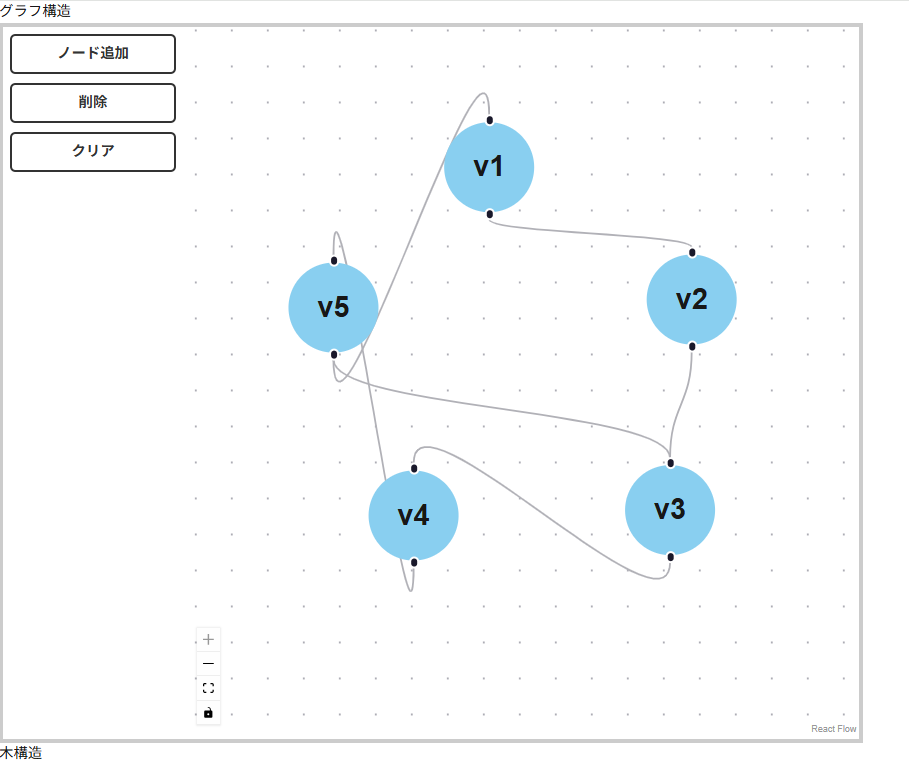
\includegraphics[scale=0.3]{graph-edit1.png}
				\caption{グラフ描画}
			\end{figure}
		\end{column}
		\begin{column}{0.04\textwidth}
			\centering
			\vrule width 0.4pt height 0.8\textheight
		\end{column}
		\begin{column}{0.48\textwidth}
			\begin{figure}
				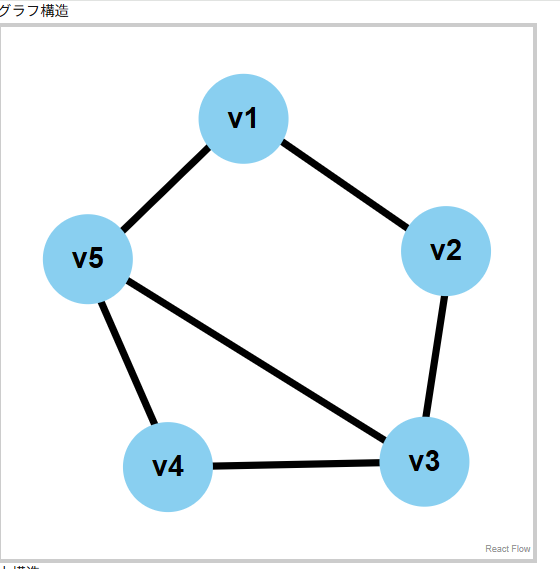
\includegraphics[scale=0.4]{graph-edit2.png}
				\caption{確認画面}
			\end{figure}
		\end{column}
	\end{columns}
\end{frame}

\section{今後の課題}
\begin{frame}{今後の課題}

\setbeamercolor{block title}{bg=purple!35, fg=black}
\setbeamercolor{block body}{bg=purple!15, fg=black}

% ---- 1つ目 ----
\begin{columns}[T,onlytextwidth]
  \begin{column}{0.72\textwidth}
    \begin{block}{問題・グラフの自動生成}
      問題内容やグラフ構造を自動的に生成し，
      学習の多様性を向上
    \end{block}
  \end{column}
  \begin{column}{0.34\textwidth}
    \centering
    
\includegraphics[width=0.5\linewidth]{AI.png}
  \end{column}
\end{columns}

\vspace{0.4em}

% ---- 2つ目 ----
\begin{columns}[T,onlytextwidth]
  \begin{column}{0.72\textwidth}
    \begin{block}{理解度分析}
      学習履歴を用いて，
      理解度やつまずきを分析
    \end{block}
  \end{column}
  \begin{column}{0.34\textwidth}
    \centering
    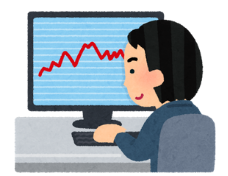
\includegraphics[width=0.6\linewidth]{analysis.png}
  \end{column}
\end{columns}

\vspace{0.4em}

% ---- 3つ目 ----
\begin{columns}[T,onlytextwidth]
  \begin{column}{0.72\textwidth}
    \begin{block}{動機付けの強化}
      ゲーム要素を導入し，
      学習意欲の向上を図る
    \end{block}
  \end{column}
  \begin{column}{0.34\textwidth}
    \centering
    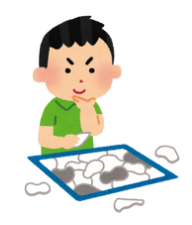
\includegraphics[width=0.6\linewidth]{puzzule.png}
  \end{column}
\end{columns}

\end{frame}
\section{まとめ}
\begin{frame}[label=sum]{まとめ}


\begin{itemize}
	\setlength{\leftskip}{-2em}
  \setlength{\parskip}{0.5em}
  \item 木幅・木分解は，一般グラフを「木に近い構造」として捉えるための重要な概念である.
  \item 定義理解の難しさに着目し，問題演習とインタラクティブ操作を通じた学習支援システムを構築した.
  \item 視覚的・操作的な学習により，木幅・木分解の直感的理解を支援できると期待される.
\end{itemize}

\end{frame}
\section{参考文献}
\begin{frame}[allowframebreaks]{参考文献}
	\renewcommand{\bibsection}{} % natbibの見出し出力を無効化する
  \footnotesize
	\bibliographystyle{plainnat}
  \bibliography{refs}
\end{frame}

\againframe{sum}
\end{document}
